\documentclass{standalone}
\usepackage{tikz}
\usetikzlibrary{patterns, positioning}
\usepackage[sfdefault]{ClearSans} %% option 'sfdefault' activates Clear Sans as the default text font
\usepackage[T1]{fontenc}

\begin{document}
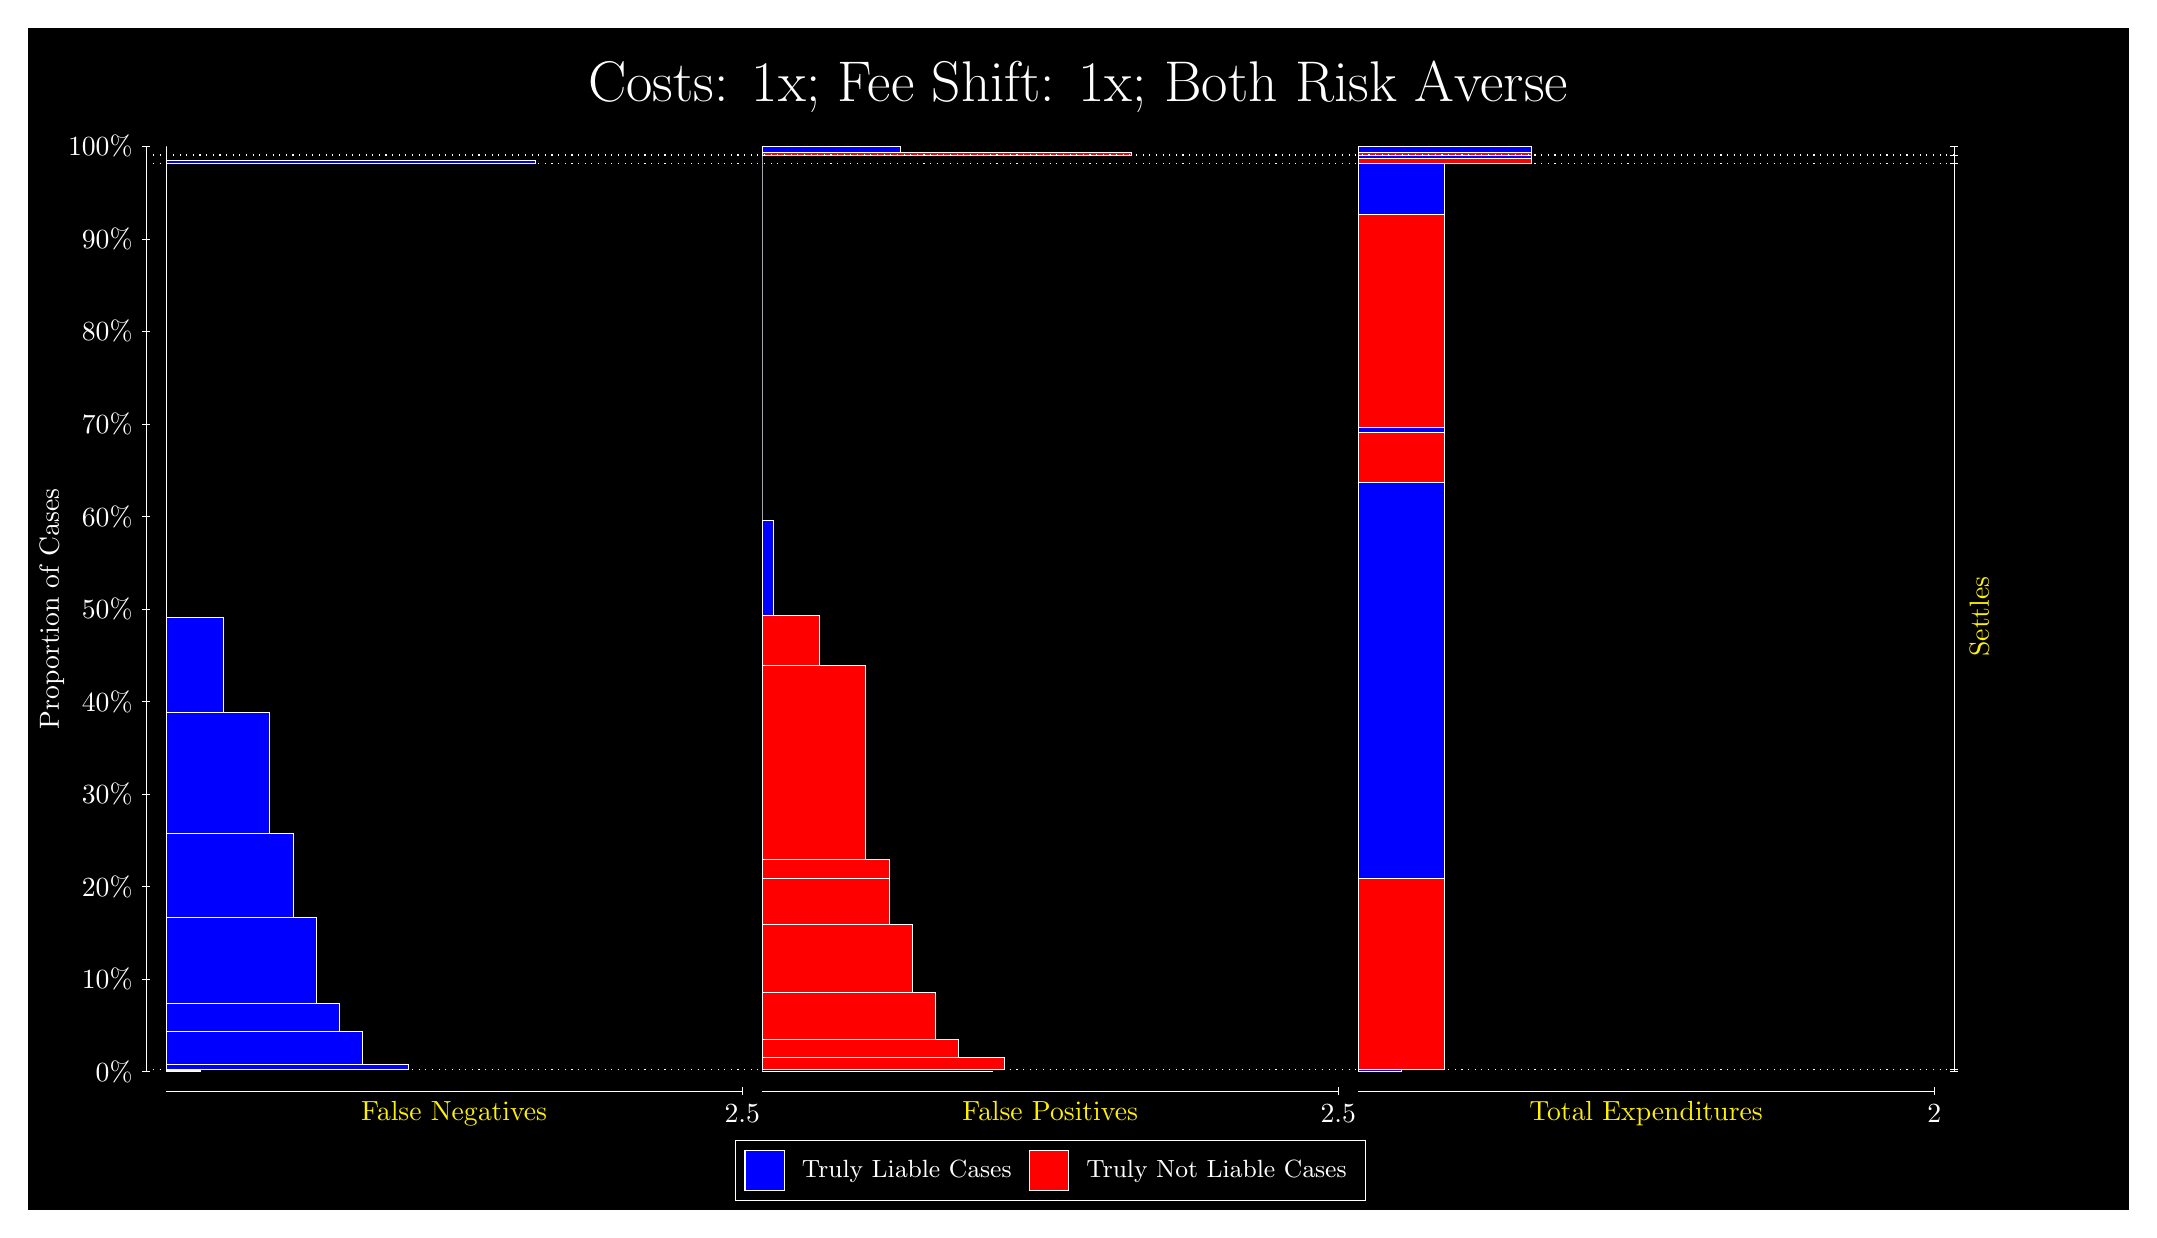
\begin{tikzpicture}
\draw[fill=black] (0,0) rectangle (26.667,15);
\draw[text=white] (0,13.5) rectangle (26.667,15) node[midway] {\huge Costs: 1x; Fee Shift: 1x; Both Risk Averse};
\draw[white, very thin] (1.5,1.75) -- (1.5,13.5);
\node[rotate=90, text=white, anchor=center] at (0.3, 7.625) {Proportion of Cases};
\draw[white, very thin] (1.45,1.75) -- (1.55,1.75);
\node[text=white, anchor=east] at (1.45, 1.75) {0\%};
\draw[white, very thin] (1.45,2.925) -- (1.55,2.925);
\node[text=white, anchor=east] at (1.45, 2.925) {10\%};
\draw[white, very thin] (1.45,4.1) -- (1.55,4.1);
\node[text=white, anchor=east] at (1.45, 4.1) {20\%};
\draw[white, very thin] (1.45,5.275) -- (1.55,5.275);
\node[text=white, anchor=east] at (1.45, 5.275) {30\%};
\draw[white, very thin] (1.45,6.45) -- (1.55,6.45);
\node[text=white, anchor=east] at (1.45, 6.45) {40\%};
\draw[white, very thin] (1.45,7.625) -- (1.55,7.625);
\node[text=white, anchor=east] at (1.45, 7.625) {50\%};
\draw[white, very thin] (1.45,8.8) -- (1.55,8.8);
\node[text=white, anchor=east] at (1.45, 8.8) {60\%};
\draw[white, very thin] (1.45,9.975) -- (1.55,9.975);
\node[text=white, anchor=east] at (1.45, 9.975) {70\%};
\draw[white, very thin] (1.45,11.15) -- (1.55,11.15);
\node[text=white, anchor=east] at (1.45, 11.15) {80\%};
\draw[white, very thin] (1.45,12.325) -- (1.55,12.325);
\node[text=white, anchor=east] at (1.45, 12.325) {90\%};
\draw[white, very thin] (1.45,13.5) -- (1.55,13.5);
\node[text=white, anchor=east] at (1.45, 13.5) {100\%};

\draw[white, very thin] (24.457,1.75) -- (24.457,13.5);
\draw[white, very thin] (24.407,1.75) -- (24.507,1.75);
\node[anchor=west] at (24.407, 1.75) {};
\draw[white, very thin] (24.407,1.7732) -- (24.507,1.7732);
\node[anchor=west] at (24.407, 1.7732) {};
\draw[white, very thin] (24.407,13.286) -- (24.507,13.286);
\node[anchor=west] at (24.407, 13.286) {};
\draw[white, very thin] (24.407,13.39) -- (24.507,13.39);
\node[anchor=west] at (24.407, 13.39) {};
\draw[white, very thin] (24.407,13.5) -- (24.507,13.5);
\node[anchor=west] at (24.407, 13.5) {};

\draw[white, very thin, fill=blue] (1.75,1.75) rectangle (2.1891,1.7708);
\draw[white, very thin, fill=red] (1.75,1.7708) rectangle (1.75,1.7732);
\draw[white, very thin, fill=blue] (1.75,1.7732) rectangle (4.8239,1.8383);
\draw[white, very thin, fill=blue] (1.75,1.8383) rectangle (4.2384,2.2551);
\draw[white, very thin, fill=blue] (1.75,2.2551) rectangle (3.9457,2.6208);
\draw[white, very thin, fill=blue] (1.75,2.6208) rectangle (3.6529,3.7063);
\draw[white, very thin, fill=blue] (1.75,3.7063) rectangle (3.3602,4.7736);
\draw[white, very thin, fill=blue] (1.75,4.7736) rectangle (3.0674,6.3069);
\draw[white, very thin, fill=blue] (1.75,6.3069) rectangle (2.4819,7.5178);
\draw[white, very thin, fill=red] (1.75,7.5178) rectangle (1.75,13.286);
\draw[white, very thin, fill=blue] (1.75,13.286) rectangle (6.4341,13.322);
\draw[white, very thin, fill=red] (1.75,13.322) rectangle (1.75,13.39);
\draw[white, very thin, fill=red] (1.75,13.39) rectangle (1.75,13.426);
\draw[white, very thin, fill=blue] (1.75,13.426) rectangle (1.75,13.5);
\draw[white, very thin, fill=red] (9.3189,1.75) rectangle (12.246,1.7524);
\draw[white, very thin, fill=blue] (9.3189,1.7524) rectangle (9.3189,1.7732);
\draw[white, very thin, fill=red] (9.3189,1.7732) rectangle (12.393,1.932);
\draw[white, very thin, fill=red] (9.3189,1.932) rectangle (11.807,2.1597);
\draw[white, very thin, fill=red] (9.3189,2.1597) rectangle (11.515,2.7624);
\draw[white, very thin, fill=red] (9.3189,2.7624) rectangle (11.222,3.6186);
\draw[white, very thin, fill=red] (9.3189,3.6186) rectangle (10.929,4.2074);
\draw[white, very thin, fill=red] (9.3189,4.2074) rectangle (10.929,4.443);
\draw[white, very thin, fill=red] (9.3189,4.443) rectangle (10.636,6.9122);
\draw[white, very thin, fill=red] (9.3189,6.9122) rectangle (10.051,7.5419);
\draw[white, very thin, fill=blue] (9.3189,7.5419) rectangle (9.4652,8.7527);
\draw[white, very thin, fill=blue] (9.3189,8.7527) rectangle (9.3189,13.286);
\draw[white, very thin, fill=red] (9.3189,13.286) rectangle (9.3189,13.354);
\draw[white, very thin, fill=blue] (9.3189,13.354) rectangle (9.3189,13.39);
\draw[white, very thin, fill=red] (9.3189,13.39) rectangle (14.003,13.426);
\draw[white, very thin, fill=blue] (9.3189,13.426) rectangle (11.075,13.5);
\draw[white, very thin, fill=red] (16.888,1.75) rectangle (17.437,1.7524);
\draw[white, very thin, fill=blue] (16.888,1.7524) rectangle (17.437,1.7732);
\draw[white, very thin, fill=red] (16.888,1.7732) rectangle (17.986,4.2074);
\draw[white, very thin, fill=blue] (16.888,4.2074) rectangle (17.986,9.2344);
\draw[white, very thin, fill=red] (16.888,9.2344) rectangle (17.986,9.8641);
\draw[white, very thin, fill=blue] (16.888,9.8641) rectangle (17.986,9.9292);
\draw[white, very thin, fill=red] (16.888,9.9292) rectangle (17.986,12.634);
\draw[white, very thin, fill=blue] (16.888,12.634) rectangle (17.986,13.286);
\draw[white, very thin, fill=red] (16.888,13.286) rectangle (19.083,13.354);
\draw[white, very thin, fill=blue] (16.888,13.354) rectangle (19.083,13.39);
\draw[white, very thin, fill=red] (16.888,13.39) rectangle (19.083,13.426);
\draw[white, very thin, fill=blue] (16.888,13.426) rectangle (19.083,13.5);
\draw[white, dotted] (1.5,1.7732) -- (24.457,1.7732);
\draw[white, dotted] (1.5,13.286) -- (24.457,13.286);
\draw[white, dotted] (1.5,13.39) -- (24.457,13.39);
\draw[white, very thin] (1.75,1.5) -- (9.0689,1.5);
\node[text=yellow, anchor=north] at (5.4094, 1.5) {False Negatives};
\draw[white, very thin] (9.0689,1.45) -- (9.0689,1.55);
\node[text=white, anchor=north] at (9.0689, 1.45) {2.5};

\draw[white, very thin] (9.3189,1.5) -- (16.638,1.5);
\node[text=yellow, anchor=north] at (12.978, 1.5) {False Positives};
\draw[white, very thin] (16.638,1.45) -- (16.638,1.55);
\node[text=white, anchor=north] at (16.638, 1.45) {2.5};

\draw[white, very thin] (16.888,1.5) -- (24.207,1.5);
\node[text=yellow, anchor=north] at (20.547, 1.5) {Total Expenditures};
\draw[white, very thin] (24.207,1.45) -- (24.207,1.55);
\node[text=white, anchor=north] at (24.207, 1.45) {2};


\node[text=yellow, centered, rotate=90] at (24.777, 7.5298) {Settles};



\draw (12.978300999999998,1.5) node[draw=none] (baseCoordinate) {};
\begin{scope}[align=center]
        \matrix[scale=0.5, draw=white, below=0.5cm of baseCoordinate, nodes={draw}, column sep=0.1cm]{
            \node[rectangle, draw, minimum width=0.5cm, minimum height=0.5cm, fill=blue] {}; &
            \node[draw=none, font=\small, text=white] (B) {Truly Liable Cases}; &
            \node[rectangle, draw, minimum width=0.5cm, minimum height=0.5cm, fill=red] {}; &
            \node[draw=none, font=\small, text=white] (B) {Truly Not Liable Cases}; \\
            };
\end{scope}

\end{tikzpicture}
\end{document}